\section{Durchführung}
\label{sec:durchfuerung}

Um die Fahrweisen in Reihen- und Parallelschaltung miteinander vergleichen zu können, würden im Präsenspraktikum verschiedene Druck-, Temperatur und Volumenstrommessungen für den warmen und den kalten Strom durchgeführt werden. Die unterschiedlichen Ventileinstellungs- und Regelungsbeschreibungen werden daher in diesem Protokoll nicht näher erläutert. Der schematische Versuchsaufbau ist in Abbildung \ref{fig:schema} dargestellt.
\vspace{2mm}

\begin{figure}[h!]
	\centering
	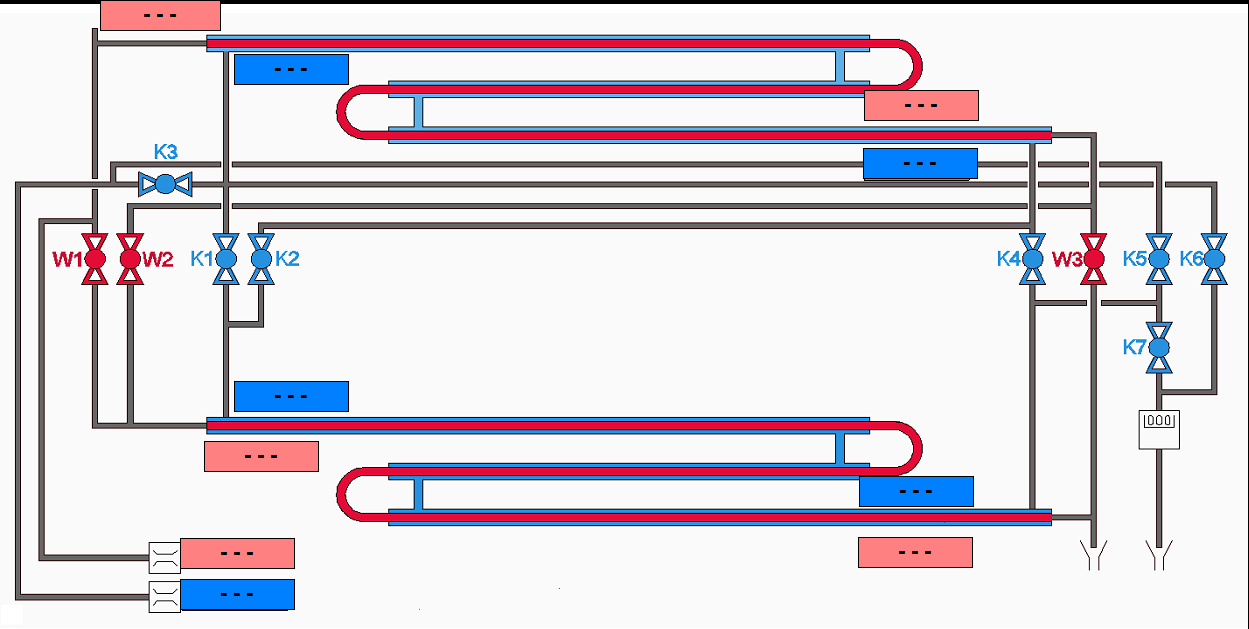
\includegraphics[width=0.8\textwidth]{img/schema}
	\caption{Schematische Darstellung des Versuchsaufbaus}
	\label{fig:schema}
\end{figure}
\FloatBarrier
%Ende